\section{Agent Interaction Protocol (AIP)} 
\label{sec:aip}
The orchestration model described in Section~\ref{sec:orchestrator} requires a communication substrate that remains \emph{correct under continuous DAG evolution}, \emph{dynamic agent participation}, and \emph{fine-grained event propagation}. Legacy HTTP-based coordination approaches (\eg A2A~\cite{duan2025agent}, ACP~\cite{ehtesham2025survey}) assume short-lived, stateless interactions, incurring handshake overhead, stale capability views, and fragile recovery when partial failures occur mid-task. These assumptions make them unsuitable for the continuously evolving workflows and long-running reasoning loops characteristic of \ufo.

\subsection{Design Overview}
\label{sec:aip:overview}
AIP serves as the \textbf{nervous system} of \ufo, connecting the ConstellationClient, device agent services, and device clients under a unified, event-driven control plane, as shown in Figure~\ref{fig:aip-overview}.
It is designed as a lightweight yet evolution-tolerant protocol to satisfy six goals: 
\begin{enumerate}[label=\textit{(G\arabic*})]
    \item Maintain persistent bidirectional sessions to eliminate per-request overhead;
    \item Unify heterogeneous capability discovery via multi-source profiling;
    \item Ensure fine-grained reliability through heartbeats and timeout managers for disconnection and failure detection;
    \item Preserve deterministic command ordering within sessions;
    \item Support composable extensibility for new message types and resilience strategies;
    \item Provide transparent reconnection and task continuity under transient failures.
\end{enumerate}

To meet these requirements, AIP adopts a persistent, bidirectional WebSocket transport and decomposes the
orchestration substrate into \textbf{five} logical strata (Figure~\ref{fig:aip-overview}), each responsible for a distinct aspect of reliability and adaptability:
\begin{itemize}[leftmargin=2em]
    \item \textbf{L1: Message Schema Layer} — Defines strongly-typed, Pydantic-validated contracts (\texttt{ClientMessage}, \texttt{ServerMessage}) for message direction, purpose, and task transitions. Structured metadata (system info, capabilities) supports unified capability discovery (\textit{G2}) and deterministic ordering via explicit ID correlation (\textit{G4}).

    \item \textbf{L2: Transport Abstraction Layer} — Provides a protocol-agnostic \texttt{Transport} interface with a production-grade WebSocket implementation supporting configurable pings, timeouts, and large payloads. Decoupled transport logic ensures low-latency persistent sessions (\textit{G1}) and future extensibility (\textit{G5}).
    
    \item \textbf{L3: Protocol Orchestration Layer} — Implements modular handlers for registration, task execution, heartbeat, and command dispatch (see Appendix~\ref{app:aip-messages}), each extending a common \texttt{AIPProtocol} base with middleware hooks (logging, metrics, auth). This design ensures ordered state transitions (\textit{G4}) and composable extensibility (\textit{G5}).
    
    \item \textbf{L4: Resilience and Health Management Layer} — Encapsulates \texttt{HeartbeatManager}, \texttt{TimeoutManager}, and \texttt{ReconnectionStrategy} with exponential backoff and automatic session recovery. It guarantees reliability (\textit{G3}) and seamless task continuity under transient disconnections (\textit{G6}).
    
    \item \textbf{L5: Endpoint Orchestration Layer} — Provides role-specific facades: \texttt{DeviceServerEndpoint}, \texttt{DeviceClientEndpoint}, and \texttt{ConstellationEndpoint}, integrating lower layers into deployable components. These endpoints unify connection lifecycle, task routing, and health monitoring across roles, reinforcing \textit{G1}–\textit{G6}.
\end{itemize}

Together, these layers form a vertically integrated stack where \textbf{L1} establishes semantic contracts, \textbf{L2} provides transport flexibility, \textbf{L3} implements protocol logic, \textbf{L4} ensures operational resilience, and \textbf{L5} delivers deployment-ready orchestration primitives. This design enables \ufo to maintain correctness and availability under DAG evolution (\textit{G4}, \textit{G5}), agent churn (\textit{G3}, \textit{G6}), and heterogeneous execution environments (\textit{G1}, \textit{G2}).


\begin{figure}[t]
    \centering
    \begin{tikzpicture}[
        node distance=0.7cm,
        % Professional layer styles with smooth gradient colors
        box/.style={
            rectangle, 
            draw=black!30, 
            line width=1pt,
            minimum width=11cm, 
            minimum height=1.2cm, 
            align=center, 
            font=\small\sffamily,
            rounded corners=3pt,
            drop shadow={shadow xshift=0.6mm, shadow yshift=-0.6mm, opacity=0.25}
        },
        % Smooth professional color scheme (soft blue-purple gradient)
        layer1/.style={box, fill=blue!8, draw=blue!40},
        layer2/.style={box, fill=blue!15, draw=blue!50},
        layer3/.style={box, fill=violet!12, draw=violet!45},
        layer4/.style={box, fill=purple!15, draw=purple!50},
        layer5/.style={box, fill=indigo!18, draw=indigo!55},
        % Professional endpoint styles
        endpoint/.style={
            box, 
            fill=teal!20, 
            draw=teal!60,
            minimum width=3cm,
            minimum height=1.05cm,
            font=\normalsize\sffamily\bfseries,
            rounded corners=4pt,
            drop shadow={shadow xshift=0.8mm, shadow yshift=-0.8mm, opacity=0.3}
        },
        % Refined arrow styles
        arrow/.style={
            ->, 
            >=stealth, 
            line width=1.3pt,
            draw=blue!55
        },
        bidir/.style={
            <->, 
            >=stealth, 
            line width=1.6pt, 
            draw=violet!50
        }
    ]
        % Layer boxes (bottom to top) with enhanced styling
        \node[layer1] (L1) at (0,0) {
            \textbf{\normalsize L1: Message Schema Layer}\\[2pt]
            {\footnotesize\texttt{ClientMessage}, \texttt{ServerMessage}, Pydantic Validation}
        };
        
        \node[layer2] (L2) [above=of L1] {
            \textbf{\normalsize L2: Transport Abstraction Layer}\\[2pt]
            {\footnotesize\texttt{WebSocketTransport}, Persistent Connections, Adapters}
        };
        
        \node[layer3] (L3) [above=of L2] {
            \textbf{\normalsize L3: Protocol Orchestration Layer}\\[2pt]
            {\footnotesize Registration, TaskExecution, Heartbeat, DeviceInfo, Command}
        };
        
        \node[layer4] (L4) [above=of L3] {
            \textbf{\normalsize L4: Resilience \& Health Management Layer}\\[2pt]
            {\footnotesize HeartbeatManager, TimeoutManager, ReconnectionStrategy}
        };
        
        \node[layer5] (L5) [above=of L4] {
            \textbf{\normalsize L5: Endpoint Orchestration Layer}\\[2pt]
            {\footnotesize DeviceServer, DeviceClient, Constellation Endpoints}
        };
        
        % Three endpoint types at the top - Device Server in the middle
        \node[endpoint] (constellation) [above=1cm of L5, xshift=-3.8cm] {
            \faSitemap\\[2pt]
            Constellation\\Client
        };
        \node[endpoint] (server) [above=1cm of L5] {
            \faServer\\[2pt]
            Device Agent \\ Server
        };
        \node[endpoint] (client) [above=1cm of L5, xshift=3.8cm] {
            \faDesktop\\[2pt]
            Device Agent \\Client
        };
        
        % Vertical arrows showing layer dependencies with subtle styling
        \draw[arrow] (L1) -- (L2);
        \draw[arrow] (L2) -- (L3);
        \draw[arrow] (L3) -- (L4);
        \draw[arrow] (L4) -- (L5);
        
        % Connection from L5 to Device Server (center)
        \draw[arrow] (L5.north) -- (constellation.south);
        \draw[arrow] (L5.north) -- (server.south);
        \draw[arrow] (L5.north) -- (client.south);
        
        % Bidirectional communication: Server connects to both clients
        \draw[bidir] (constellation.east) -- (server.west);
        \draw[bidir] (server.east) -- (client.west);
        
        % Add a subtle decorative border around the entire stack
        \draw[draw=gray!25, line width=0.6pt, rounded corners=6pt]
            ([xshift=-0.4cm, yshift=-0.35cm]L1.south west) rectangle 
            ([xshift=0.4cm, yshift=0.35cm]L5.north east);
        
    \end{tikzpicture}
    \caption{AIP Architecture: Five-layer protocol stack enabling persistent, resilient multi-agent orchestration.}
    \label{fig:aip-overview}
\end{figure}


\subsection{Agent Registration and Profiling}
\label{subsec:aip-registration}

Agent registration in AIP corresponds to the entry point of the orchestration pipeline, anchoring the capability discovery and topology formation processes outlined in \textit{(G2)} and implemented primarily through the \textbf{L1–L3 layers}.
\begin{figure}[t]
  \centering
  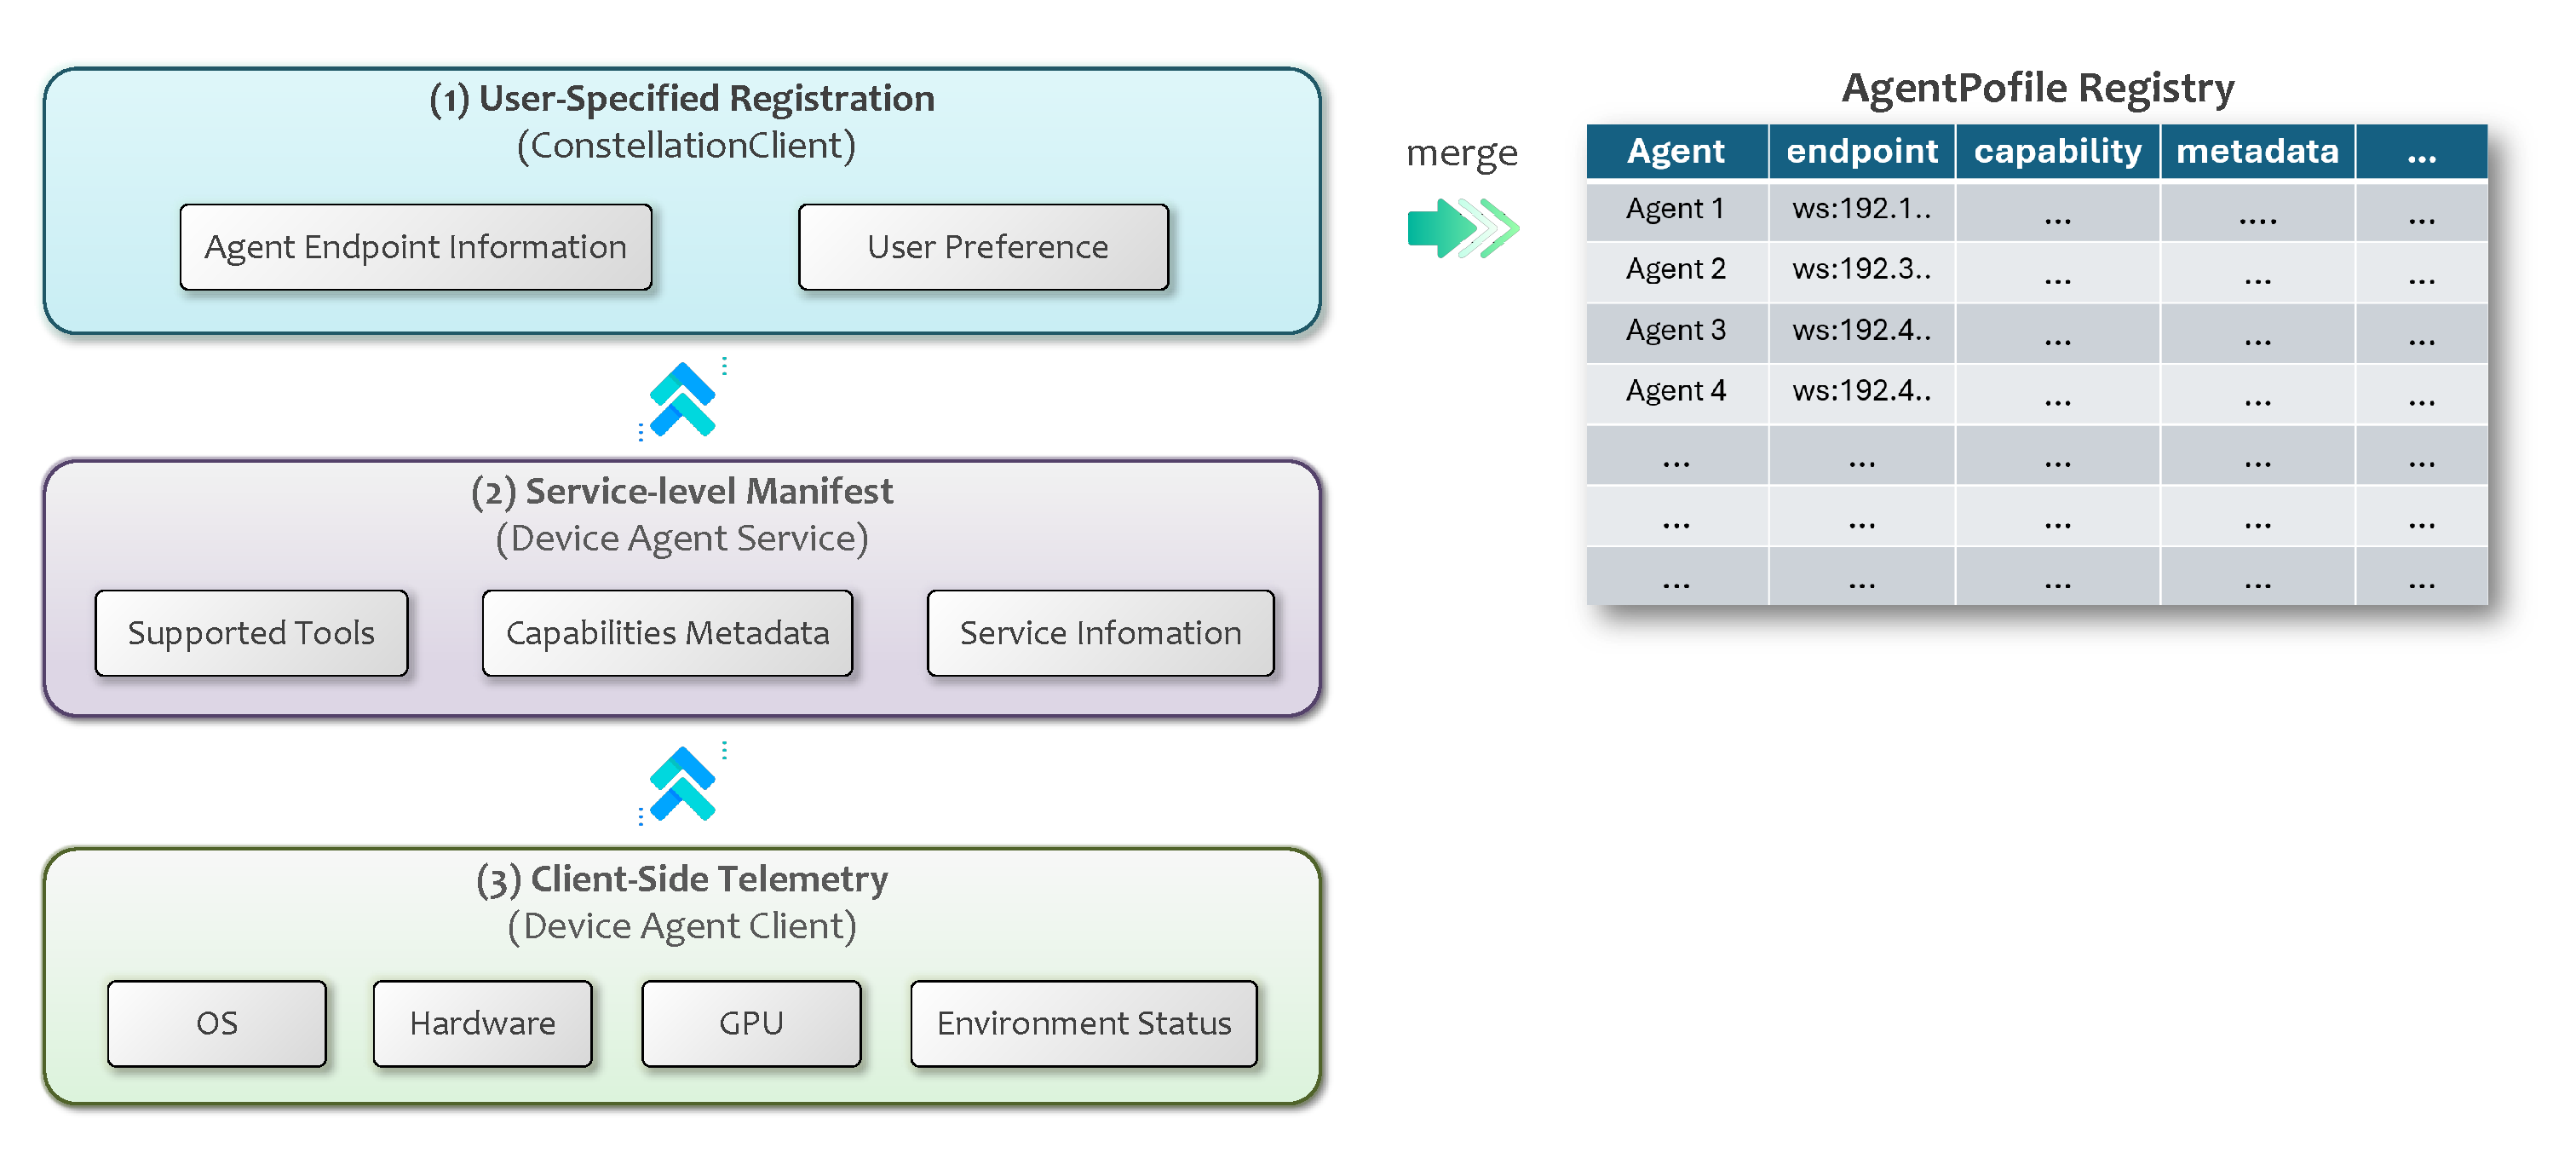
\includegraphics[width=\textwidth]{images/agent_registry.pdf}
  \vspace{-2em}
  \caption{Agent registration flow: multi-source AgentProfile construction and registration.}
  \label{fig:agent-registration}
\end{figure}

As illustrated in Figure~\ref{fig:agent-registration}, the registration pipeline consists of three complementary stages that together establish a unified and continuously refreshed view of the constellation's capabilities:
\begin{enumerate}
    \item \textbf{User-specified registration (ConstellationClient).} Administrators provide endpoint identities and specify user preferences. These initial configurations define the logical boundaries of the constellation and seed the connection parameters required for session establishment.
    
    \item \textbf{Service-level manifest (device agent service).} Each device agent advertises its supported tools, environment variables, and operational metadata through a \texttt{REGISTER} message. These descriptors are validated and normalized by the \textbf{Message Schema Layer (L1)} and merged through the \textbf{Protocol Orchestration Layer (L3)}, ensuring semantic consistency and structured capability discovery.
    
    \item \textbf{Client-side telemetry (device agent client).} Local clients continuously report runtime metrics, such as OS version, hardware status, GPU utilization, and software environment, to the device agent service. This telemetry stream keeps the global registry up to date and enables adaptive re-scheduling under resource drift or device churn.
\end{enumerate}

\begin{figure}[t]
\centering
\scalebox{0.85}{
\begin{tcolorbox}[
  enhanced,
  width=0.92\linewidth,
  colback=CardBG,
  colframe=CardBorder,
  boxrule=0.4pt,
  arc=2mm,
  sharp corners=south,
  drop shadow=black!10
]
% Header
\begin{tikzpicture}[font=\sffamily]
\node (title) at (0,0) [anchor=west, text=Accent] {\Large \textbf{AgentProfile:} \texttt{gpu\_agent}};
\node (status) [right=1cm of title, anchor=west, draw=CardBorder,
  rounded corners=2pt, inner xsep=6pt, inner ysep=2pt] 
  {\textbf{Status:} \textcolor{Good}{idle}};
\end{tikzpicture}

\vspace{4pt}\hrule height0.4pt \color{CardBorder}\vspace{6pt}

% Body: two columns
\begin{minipage}[t]{0.48\linewidth}
\textbf{System}\\
OS: \texttt{linux} \quad(\texttt{Ubuntu 24.04})\\[2pt]
Capabilities: \texttt{cli}, \texttt{file\_system}, \texttt{data\_processing}, \texttt{model\_training}\\[6pt]

\textbf{Paths}\\
Dataset: \texttt{\textasciitilde/dataset}\\
Training: \texttt{\textasciitilde/script}\\
Code: \texttt{\textasciitilde/code}\\
\end{minipage}\hfill
\begin{minipage}[t]{0.48\linewidth}
\textbf{Performance}\\
GPU: \texttt{4 $\times$ NVIDIA A100 80G}\\
CPU: \texttt{96 cores}\\
Memory: \texttt{866.1 GB}\\[6pt]

\textbf{Network \& Host (optional)}\\
Host: \texttt{gui-model-a100}\\
IP: \texttt{172.19.0.4}
\end{minipage}

\vspace{6pt}\hrule height0.4pt \color{CardBorder}\vspace{4pt}
{\footnotesize Last heartbeat: 2025-10-28 07:46:24 UTC\quad | \quad Server: \texttt{ws://localhost:5005/ws}}
\end{tcolorbox}
}
\caption{An example \textbf{AgentProfile} of a GPU agent with Linux system.}
\label{fig:agentprofile-card}
\end{figure}


The aggregated results from these three stages are merged by the ConstellationClient into a unified \textit{AgentProfile} that represents each agent's real-time operational state. An example \textit{AgentProfile} for a GPU-enabled device is shown in Fig.~\ref{fig:agentprofile-card}, demonstrating how multi-level profiling captures hardware, software, and dynamic runtime descriptors within a single schema.

Through this registration and profiling pipeline, AIP achieves continuous capability discovery, evolution-tolerant orchestration, and consistent topology awareness across heterogeneous devices. The process directly fulfills \textit{(G1–G3)} by maintaining persistent sessions, ensuring reliable metadata propagation, and enabling transparent adaptation as the constellation evolves.

\subsection{Task Dispatch and Result Delivery}
\label{subsec:aip-dispatch}
Task dispatch operationalizes the event-driven execution model envisioned in \textit{(G1)} and \textit{(G4)} through tightly managed sessions that persist across multiple task rounds. When the ConstellationClient assigns a \TaskStar to a device, the Transport Abstraction Layer guarantees low-latency delivery of the serialized \texttt{TASK} message to the target agent service. The Protocol Orchestration Layer coordinates message routing, while the Resilience and Health Management Layer monitors the session heartbeat to ensure reliability.

Each task follows a deterministic life cycle, from \texttt{TASK} to \texttt{TASK\_END}, with strict ordering guarantees enforced by the session-level sequence manager. Intermediate logs and evaluator outputs are streamed back incrementally to the ConstellationClient, which updates the global \TaskConstellation state and triggers potential DAG adjustments.

This continuous, feedback-driven execution loop transforms AIP from a mere transport protocol into a temporal coordination substrate, harmonizing asynchronous reasoning, scheduling, and execution across distributed devices.

\subsection{Command Execution}
\label{subsec:aip-commands}
At a finer operational granularity, AIP implements a unified \textbf{command execution model} that directly fulfills \textit{(G4)} and \textit{(G5)} by ensuring deterministic, extensible control within persistent sessions.

Each \texttt{COMMAND} message specifies a unique identifier, target function, and a typed argument list. The Message Schema Layerenforces structure and validation, while the Protocol Orchestration Layer executes commands sequentially within the session context to maintain determinism. To optimize multi-action workflows, multiple commands may be batched in a single message, reducing round-trip overhead. Execution results are returned as structured \texttt{Result} objects, containing status codes, return values, and error metadata. Failures or timeouts are propagated through the same channel, enabling the orchestrator to apply adaptive recovery or task reassignment strategies via \textbf{L4}'s resilience mechanisms.

Unified with \ufo's MCP tool-calling interface, this model bridges system-level orchestration with model-generated actions, ensuring that high-level reasoning and low-level execution operate under a consistent and evolvable protocol surface.

\subsection{Resilient Connection Protocol}
\label{subsec:aip-resilience}

The distributed and volatile nature of device environments necessitates a dedicated resilience layer to uphold \textit{(G3)} and \textit{(G6)}. AIP's \textbf{Resilient Connection Protocol}, implemented primarily within \textbf{L4}, guarantees synchronized fault handling and seamless recovery across client–server boundaries.

When a \textit{Device Agent} disconnects unexpectedly, the orchestrator immediately marks it as \texttt{DISCONNECTED}, removes it from the active scheduling pool, and triggers background reconnection attempts using exponential backoff. Upon recovery, the agent re-registers automatically, restoring its prior session state and resuming task participation without manual intervention.
If disconnection occurs during task execution, all affected tasks are transitioned to \texttt{TASK\_FAILED}, and corresponding updates are propagated to the \cagent for DAG revision, ensuring that the orchestration view remains globally consistent.

Symmetrically, when the \textit{ConstellationClient} itself disconnects, the corresponding \textit{Device Agent Server} receives a termination signal and \emph{proactively aborts} all ongoing tasks associated with that client. This bidirectional fault-handling policy prevents resource leakage, avoids orphaned execution states, and guarantees that both endpoints maintain a consistent global view of task progress.

Together, these mechanisms realize an end-to-end resilient orchestration substrate that preserves correctness, availability, and synchronization under transient network failures or partial system outages,closing the reliability loop envisioned in AIP's layered design.

\paragraph{Summary.}
AIP consolidates registration, task dispatch, command execution, and resilience into a coherent, evolution-tolerant communication fabric that embodies the six goals outlined in Section~\ref{sec:aip:overview}. Functionally, AIP forms the \textbf{nervous system of \ufo}, enabling reasoning, execution, and recovery to operate seamlessly within an evolving constellation of intelligent agents. Its minimal yet extensible design ensures that as workflows, models, and environments evolve, the underlying communication protocol remains stable, adaptive, and correct by construction.
